\begin{center}
\begin{tikzpicture}
    \node[anchor=south west,inner sep=0] (image)  at (0,0) {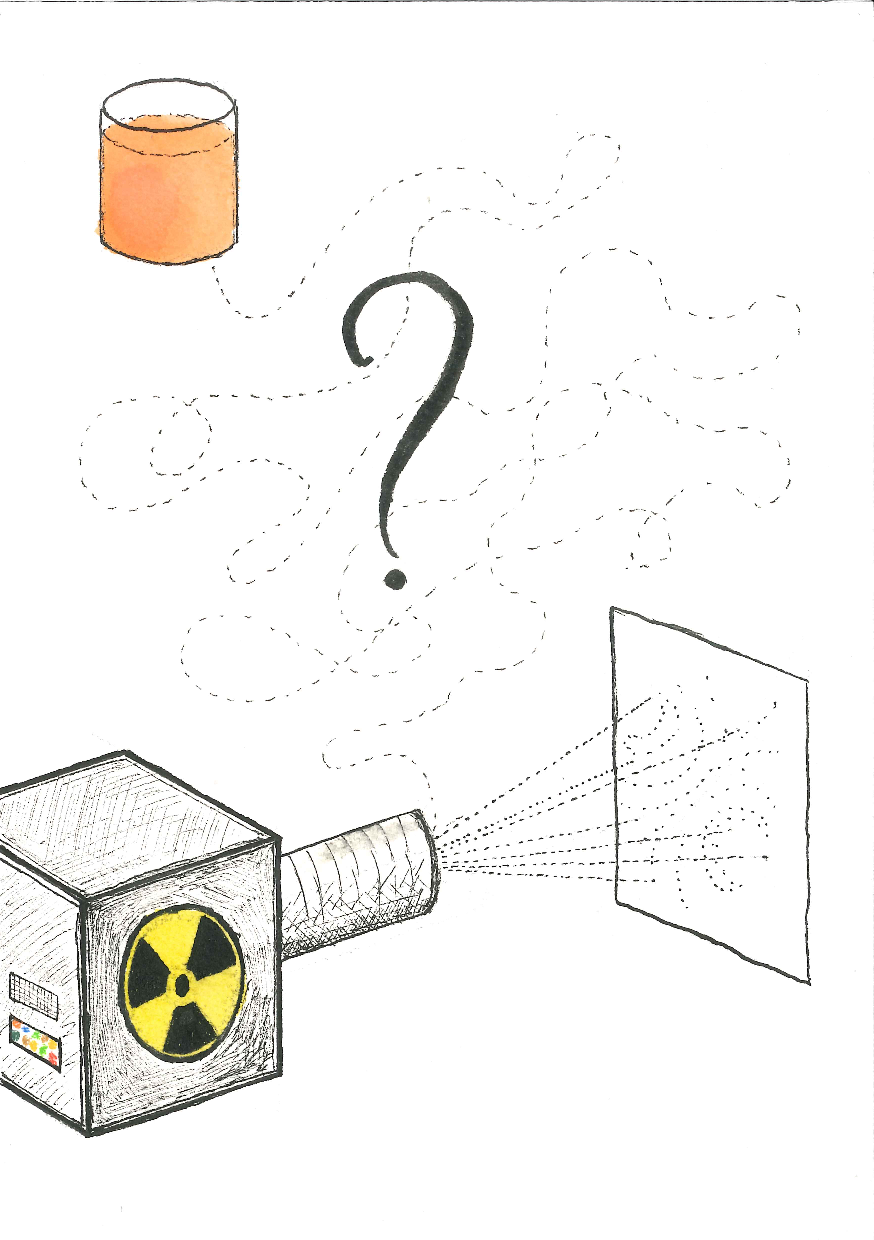
\includegraphics[trim={2mm, 2mm, 2mm, 2mm}, width=0.995\pagewidth]{scans/pg_0004.pdf}};
    
    \begin{scope}[x={(image.south east)},y={(image.north west)}]
        \if\helplines1
        	\draw[help lines,xstep=.1,ystep=.1] (0,0) grid (1,1);
        \fi
        \node[align=justify, anchor=north west, text width=0.35\pagewidth] at (0.55, 0.9) {\english{But the path to obtain a three-dimensional structure is long and tortuous, and often fails.
        
        \vspace{1em}
        
        \doindent Obtaining the structure of a single human protein can cost several millions.
        }};
        
        \node[align=justify, anchor=north west, text width=0.35\pagewidth] at (0.05, 0.6){\spanish{Pero el proceso para obtener la estructura tridimensional es largo, tortuoso y repleto de fallos.
        
        \vspace{1em}
        
        \doindent Obtener la estructura de una sóla proteína humana puede costar millones.
        }};
    \end{scope}

\end{tikzpicture}
\end{center}